\documentclass[12pt]{article}
\usepackage{sbc-template}
\usepackage{graphicx,url}
\usepackage[brazil]{babel}
\usepackage[utf8]{inputenc}
\usepackage{paralist}
\usepackage{graphicx}
\usepackage{subfig}
\usepackage{tabularx}

\sloppy

\title{Detecção de padrões de legendas em imagens de ritmo visual a partir
do detector de Harris}

\author{Guilherme Polo\inst{1}, Miguel Gaiowski\inst{1}}

\address{Instituto de Computação -- Universidade Estadual de Campinas
  (UNICAMP)\\
  Caixa Postal 6176 -- 13083-852 -- Campinas -- SP -- Brazil
  \email{\{ggpolo,miggaiowski\}@gmail.com}
}


\begin{document}
\maketitle

\begin{resumo}
  Vazio.
\end{resumo}


\section{Introdução}

\cite{harris}


\section{O detector de Harris}

\begin{figure}[h]
  \centering
  \subfloat[blah]{
\includegraphics[height=4cm]{figs/sample_9_9.png}}\quad
  \subfloat[bleh]{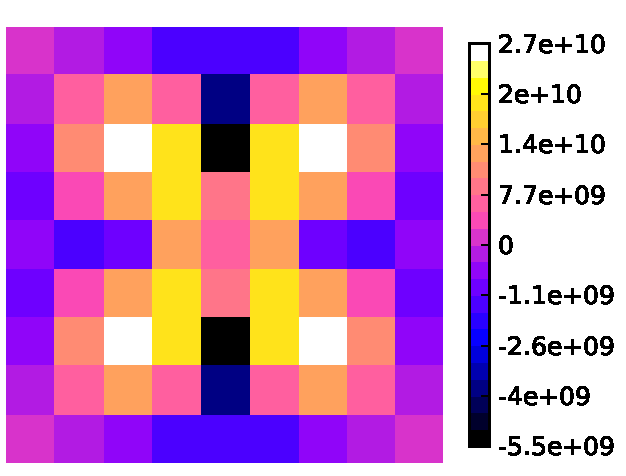
\includegraphics[height=4cm]{figs/sample_9_9_R}}
  \caption{legal}
\end{figure}


\section{Implementação}

\section{Avaliação}

\section{Conclusão}


\bibliographystyle{sbc}
\bibliography{biblio}

\end{document}
